\chapter{Einleitung}

\begin{itemize}
    \item Schüttgutsortierung ist ein wichtiges Thema \todo{hier vielleicht dieses 10\% der Energie Beispiel bringen?}
    \item Anwendungsbereiche Schüttgutsortierung
    \item Maschinelle Lernverfahren sind ein heißes Thema, dass bei vielen existierenden problemen Anwendung findet
\end{itemize}

Schüttgüter und ihr Transport sind aus unserer modernen, globalisierten Welt nicht mehr wegzudenken.
Ob es sich um Lebensmittel wie Getreide, Kaffeebohnen oder Zucker, Bergbauerzeugnisse wie Eisenerze oder Kohle, oder [Granulat/Pellets] handelt, 
[...]
[nicht-destruktiv]
In dieser Arbeit soll es insbesondere um die bilddatenbasierte beziehungsweise optische Schüttgutsortierung gehen.



\todo{Einleitungstext}

\section{Motivation}

\color{blue}
\begin{itemize}
    \item State of the Art: große Sortierer 
    \item Kooperation ISAS IOSB, \textit{TrackSort} Projekt 
    \item Flächenkamera
    \item 2 geteiltes Problem: Tracking und Prediction
    \item Fokus dieser Arbeit: Prediction
    \item Bewegungsmodelle für verschiedene Schüttgüter von Hand finetunen ist viel Aufwand und schwer
    \item Option: Neuronale Netze einsetzen! 
    \item zwei verschiedene Problemstellungen:
    \item 1. die Position des Teilchens im nächsten Zeitschritt. \textbf{NextStep} für Trackingphase
    \item 2. die Position (und die Zeit) die das Teilchen beim Passieren des Düsenarrays haben wird. \textbf{Separator}
    \item Aktuell: auf Messungen - kein Vollständiger Schätzer
\end{itemize}
\color{black}

\todo[inline]{arbeit motivieren. Schüttgutsortierung ist ein interessantes Feld, das sich potenziell für ML anbietet.}
\todo[inline]{auf jeden fall separator- und NextStep-Netze unterscheidung erwähnen}

Der Großteil der heute in der Industrie eingesetzten optischen Schüttgutsortierer verwenden Zeilenkameras.
Diese haben jedoch den Nachteil, dass die Annahme getroffen werden muss, dass die Schüttgutpartikel keinerlei Geschwindigkeit orthogonal zur Transportrichtung haben.
In Abbildung~\ref{fig:predMissed} ist dargestellt wie es, wenn diese Annahme verletzt wird, zu einer Fehlseparierung kommen kann.
Durch den Einsatz von Flächenkameras ist es möglich die Position eines Partikels auf dem Förderband zu mehreren Zeitpunkten zu bestimmen.
Basierend auf diesen Informationen sollen die Trajektorien der einzelnen Partikel vorhergesagt werden.
Diese sollen dazu verwendet werden um die Sortierqualität zu steigern. 
Im Rahmen des \textit{TrackSort} Projekts, 
einer Kooperation zwischen dem Lehrstuhls für Intelligente Sensor-Aktor-Systeme (ISAS) des Karlsruher Instituts für Technologie
und dem Fraunhofer-Institut für Optronik, Systemtechnik und Bildauswertung (IOSB), 
wurde die Verbesserung der Schüttgutsortierung durch den Einsatz von Trackingverfahren betrachtet.

\begin{figure}[h]
    \centering
    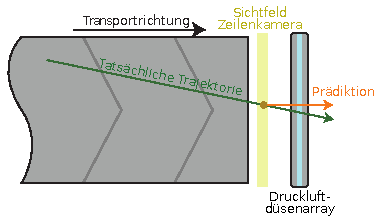
\includegraphics[width=0.8\textwidth]{PredictionMissed_translated.pdf}
    \caption{Darstellung einer Fehlseparierung durch die Annahme, dass es keine Bewegung orthogonal zur Transportrichtung gibt. 
    Übersetzt aus~\cite{Pfaff2018}.}
    \label{fig:predMissed}
\end{figure}


Um die zukünftigen Trajektorien der Partikel aus den vergangenen Positionen vorherzusagen existieren verschiedene Bewegungsmodelle, 
die je nach Situation -- Bandgeschwindigkeit, Schüttguttyp, Prädiktionsdistanz -- unterschiedlich gute Ergebnisse liefern.  
In dieser Arbeit soll erforscht werden, ob der Einsatz von Maschinellem Lernverfahren zu einer Verbesserung dieser Ergebnisse führen kann.
Dabei wird exemplarisch am \textit{TableSort} Schüttgutsortier gearbeitet.

Dafür sollen im Rahmen dieser Arbeit zwei verschiedene Prädiktionsprobleme durch neuronaler Netze gelöst werden.
Einerseits soll vorhergesagt werden, an welcher Position sich ein Teilchen im nächsten Zeitschritt befinden wird.
Solche Netze werden von hier an als NextStep-Netze bezeichnet.
Eine Visualisierung dieser Aufgabe ist in Abbildung~\ref{fig:visualsNextstep} zu sehen.
Dies hilft dabei das Zuordnungsproblem bei Trackingverfahren zu lösen.
Andererseits soll vorhergesagt werden an welcher Position und wann ein Teilchen das Druckluftdüsenarray passieren wird.
Diese Problemstellung wird von sogenannten Separator-Netzen gelöst.
Eine Visualisierung dieser Aufgabe ist in Abbildung~\ref{fig:visualsSeparator} zu sehen.
Die Qualität dieser Prädiktion ist ausschlaggebend für den Erfolg der Separation.


\begin{figure}[h]
    \centering
    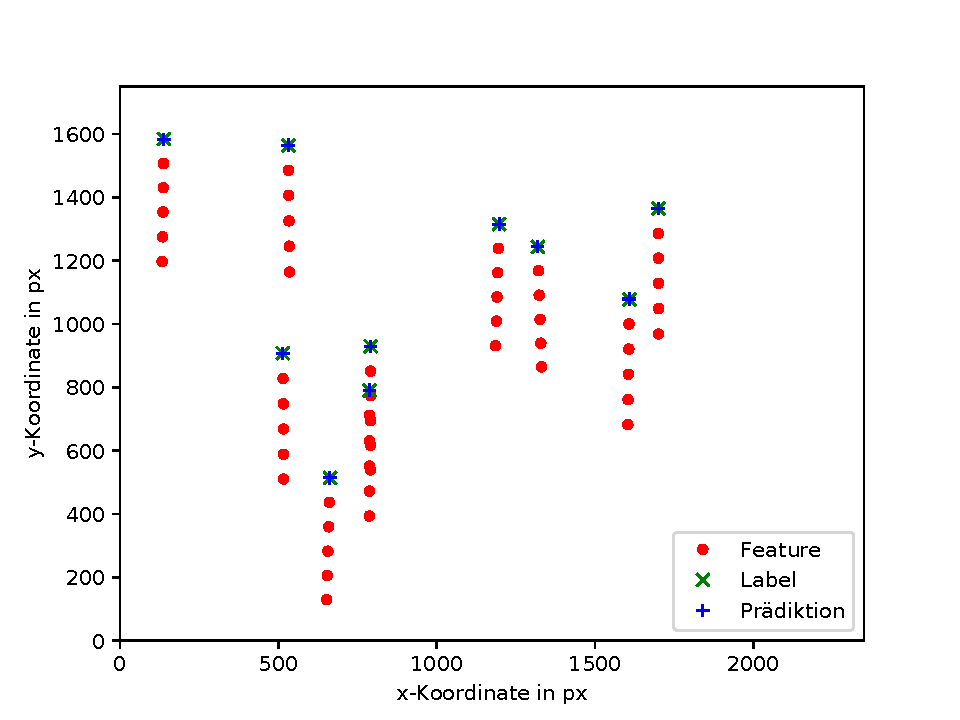
\includegraphics[width=0.8\textwidth]{NextStep-45kDecaySteps-ZylinderReal_2018-11-29.pdf}
    \caption{Visualisierung einer gelösten Probleminstanz eines NextStep-Netzes.}
    \label{fig:visualsNextstep}
\end{figure}


\begin{figure}[h]
    \centering
    % \missingfigure{Real_Weizen_final_separatorExample.pdf}
	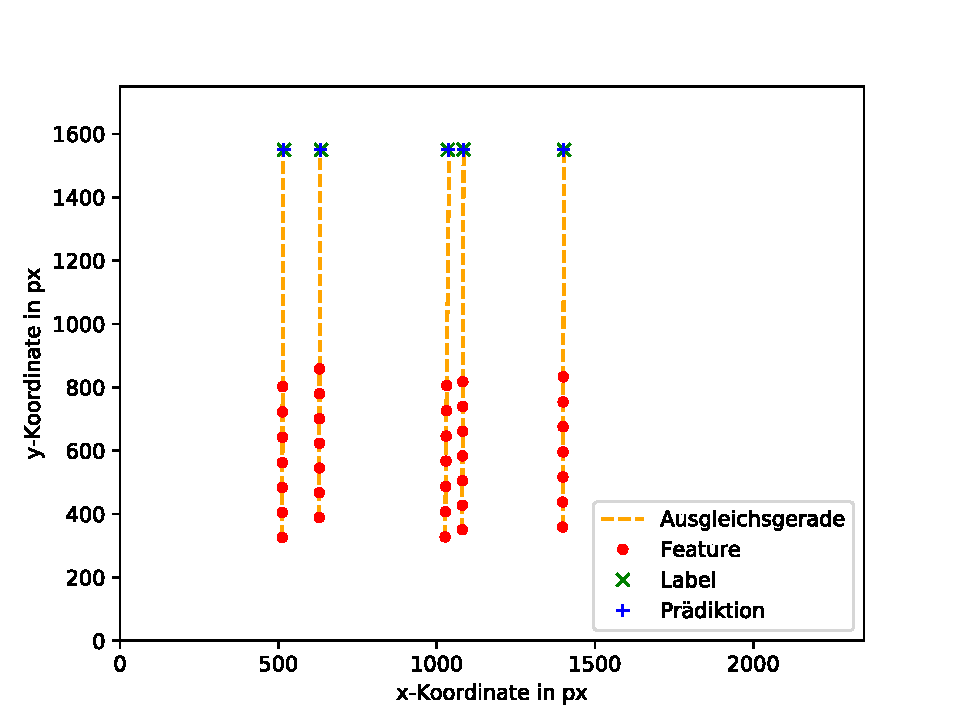
\includegraphics[width=0.8\textwidth]{Real_Weizen_final_separatorExample.pdf}
	\caption{Visualisierung einer gelösten Probleminstanz eines Separator-Netzes.}
	% \todo{Quelle Bild!}
	\label{fig:visualsSeparator}
\end{figure}



\section{Aufbau der Arbeit}

Das schreibe ich auf, wenn die Gliederung finalisiert ist.

\todo{aufbau Gliederung beschreiben. Ganz am Ende dann, wenn sich nichts mehr ändert}

